\chapter{Strumenti numerici indicatori - parte VII}

\begin{figure}[h]
    \centering
    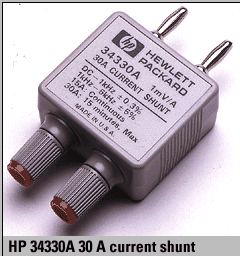
\includegraphics[scale = 1.5]{HP current shunt.png}
\end{figure}

\newpage    

\section{Voltmetro + Amperometro}
\footnote{Slide della prof | SDME 4 Strumenti numerici indicatori - parte VII | pag 3 \\  
Appunti | 2025-05-20 | pag 3 }

Dai capitoli precedenti, sappiamo la struttura dell'architettura interna di un voltmetro + amperometro. \newline 

Rispetto alle boccole dello strumento reale, i collegamenti sono i seguenti: 

\begin{figure}[h]
    \centering
    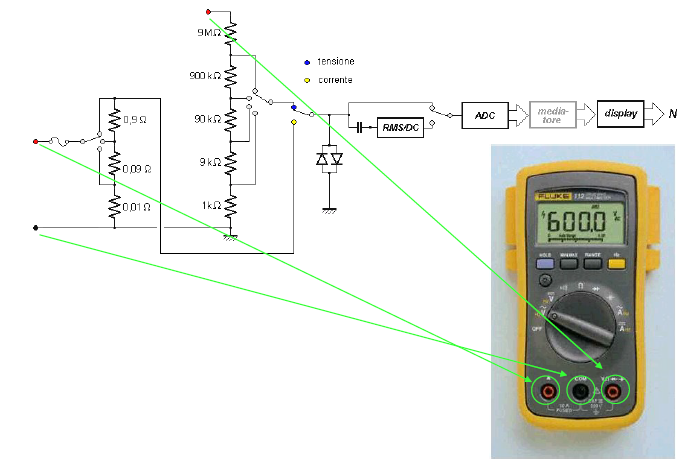
\includegraphics[scale = 1]{Voltmetro + amperometro boccole rispetto all'architettura.PNG}
\end{figure}

\newpage 

\subsection{Portate massime tipiche di voltmetro e amperometro}
\footnote{Slide della prof | SDME 4 Strumenti numerici indicatori - parte VII | pag 4 - 5\\  
Appunti | 2025-05-20 | pag 3 }

Come abbiamo studiato dai capitoli precedenti, per gli usi comuni, i tester hanno portate molto elevate. \newline 

Di seguito le caratteristiche di un Fluke 112: 

\begin{figure}[h]
    \centering
    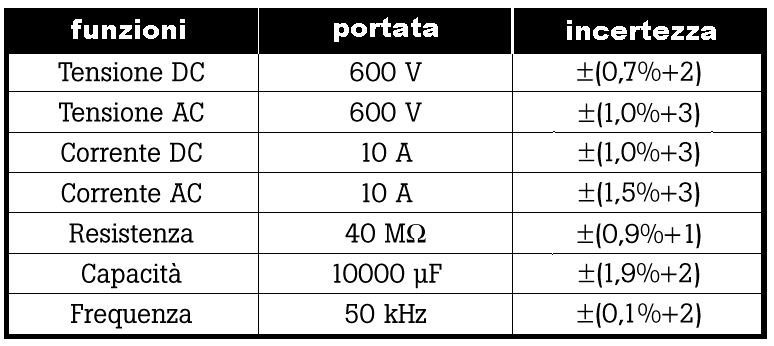
\includegraphics[scale = 0.5]{Specifiche Fluke 112.png}
\end{figure}

Ma, per quanto riguarda gli usi industriali, i tester operano con tensioni, correnti e potenze limitate, soprattutto perchè si vuole garantire la sicurezza 
dell'operatore che utilizza lo strumento. \newline 

Anche per uno strumento da banco come l'Agilent 34401A, le caratteristiche indicate nei boccoli per tensione e corrente sono le seguenti: 

\begin{itemize}
    \item $V_{max}$ in DC: 1000 V 
    \item $V_{max}$ in AC: 700 V
    \item $I_{max}$ in DC: 3 A 
    \item $I_{max}$ in AC: 3 A
\end{itemize}

\newpage 

\section{Accoppiamento diretto (DC - Direct Coupling ): Sonde per Alta Tensione e resistori Shunt}
\footnote{Slide della prof | SDME 4 Strumenti numerici indicatori - parte VII | pag 6\\  
Appunti | 2025-05-20 | pag 3 }

Se abbiamo necessità di misurare tensioni elevate, ci vengono in aiuto le sonde per l'alta tensione come le seguenti: 

\begin{figure}[h]
    \centering
    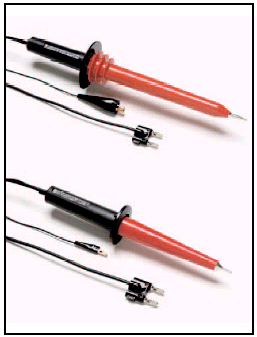
\includegraphics[scale = 0.8]{Sonde per l'alta tensione.png}
\end{figure}

oppure i resistori di shunt come il seguente: 

\begin{figure}[h]
    \centering
    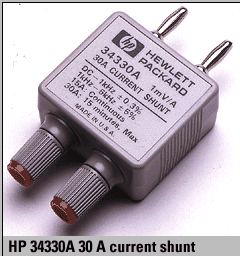
\includegraphics[scale = 0.8]{HP current shunt.png}
\end{figure}

Come si denota dalla descrizione dello Shunt dell'HP, 
uno shunt di corrente supporta correnti molto elevate (in questo modello fino a 30 A). \newline 

\newpage 

\section{Sonde per Alta Tensione}
\footnote{Slide della prof | SDME 4 Strumenti numerici indicatori - parte VII | pag 7 - 9\\  
Appunti | 2025-05-20 | pag 3 }

Prendendo un esploso della sonda per alta tensione, il Fluke 80k-40: 

\begin{figure}[h]
    \centering
    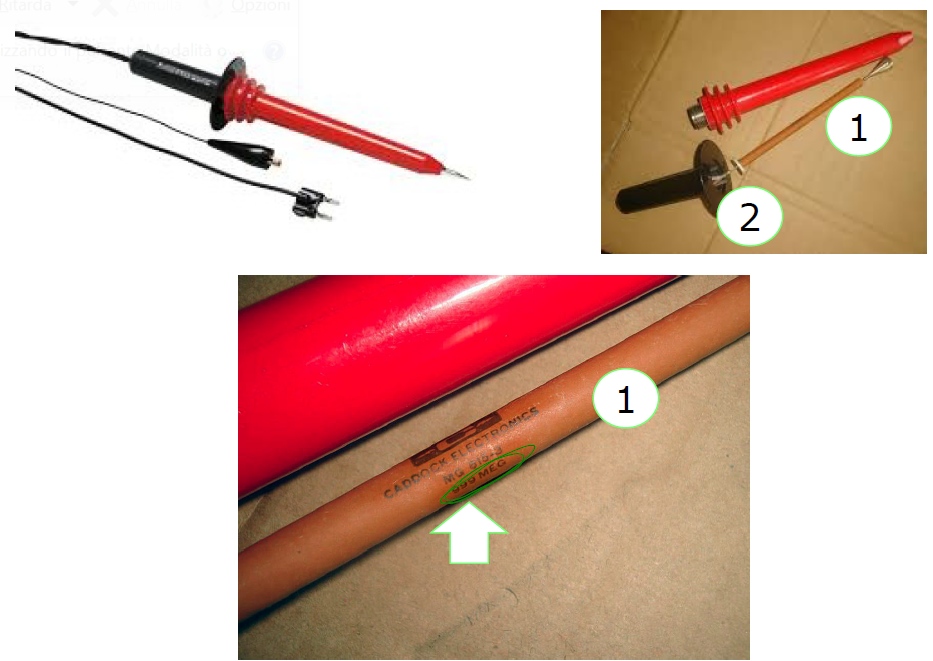
\includegraphics[scale = 0.8]{Esploso Fluke 80k-40.PNG}
\end{figure}

e confrontando il circuito ideale della sonda: 

\begin{figure}[h]
    \centering
    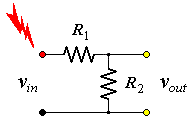
\includegraphics[scale = 2]{circuito sonda per alta tensione.png}
\end{figure}

$R_1$ è la guaina esterna dalla sonda (indicato in figura con il numero 1), con valore nominale di 999 M$\Omega$, 
invece il filo interno (indicato in figura con il numero 2), è la resistenza $R_2$ con valore nominale di 1 M$\Omega$. \newline 

Se consideriamo la sonda a vuoto, quindi senza un carico in parallelo a $R_2$, 
il circuito è un banale partitore di tensione dove, sostiutendo i valori nominali della sonda:

{
    \Large 
    \begin{equation}
        \begin{split}
            v_{out} 
            &= \frac{R_2}{R_1 + R_2} \cdot v_{in}
            \\
            &= \frac{1 M\Omega}{999 M\Omega + 1 M\Omega} \cdot v_{in}
            \\
            &= \frac{1}{1000} \cdot v_{in}
        \end{split}
    \end{equation}
}

Ma, se dobbiamo fare una misura della tensione $v_{out}$, 
come abbiamo studiato precedente, 
la resistenza $R_{in}$ di ingresso di un voltmetro è di 10 M$\Omega$. \newline 

Quindi non vale la espressione di $v_{out}$ a vuoto perchè il nuovo circuto di misura sarà il seguente: 

\begin{figure}[h]
    \centering
    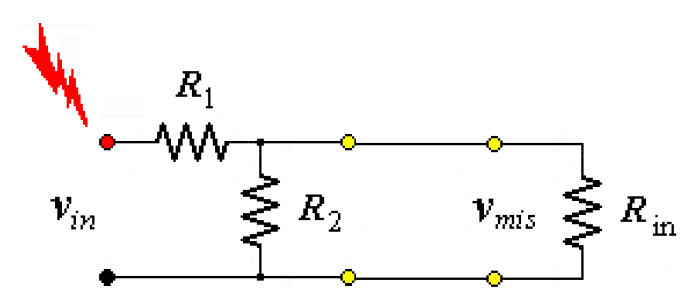
\includegraphics[scale = 1]{circuito di misura per sonda ad alta tensione.PNG}
\end{figure}

$v_{out}$ non sarà quella ai capi di $R_2$, ma sarà la tensione ai capi di $R_2$ in parallelo a $R_{in}$. \newline 

$v_{mis}$ sarà uguale a: 

{
    \Large
    \begin{equation}
        \begin{split}
            v_{mis}
            &= 
            \frac{R_2 // R_{in}}{R_1 + (R_2 // R_{in})} \cdot v_{in}
            \\
            &= 
            \frac{\frac{R_2 \cdot R_{in}}{R_2 + R_{in}}}{R_1 + \frac{R_2 \cdot R_{in}}{R_2 + R_{in}}} \cdot v_{in}
        \end{split}
    \end{equation}
}

Dal mitico corso dei RadioAmatori (questa è una chicca solo per pochi eletti), 
sappiamo che sicuramente la resistenza $R_2 // R_{in}$ sarà minore della resistenza più piccola tra i due resistori in parallelo, 
in questo caso $R_2 // R_{in}$ sarà più piccola di $R_2$. \newline 

\newpage 

\subsection{Sonde per Alta Tensione e voltmetro}
\footnote{Slide della prof | SDME 4 Strumenti numerici indicatori - parte VII | pag 10\\  
Appunti | 2025-05-20 | pag 4 }

Il circuito finale in cui la sonda ad alta tensione è collegata al voltmetro è la seguente: 

\begin{figure}[h]
    \centering
    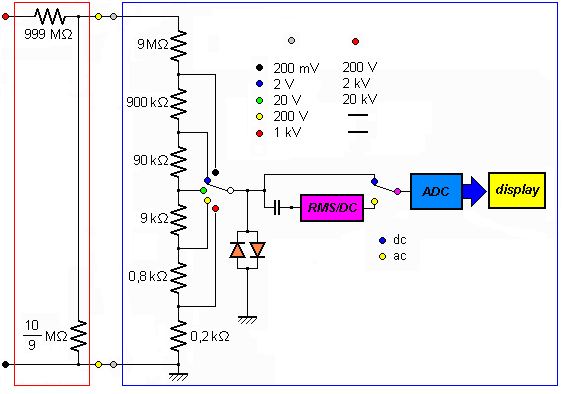
\includegraphics[scale = 1]{Architettura pinza per alta tensione e voltmetro.png}
\end{figure}

dove, fisicamente, la porzione di circuito tratteggiata in rosso è la sonda, 
invece quella porzione di circuito tratteggiata in blu è il voltmetro. \newline 

Notiamo però una cosa anomala: il valore della resistenza in parallelo alla resistenza della guaina non è più 1 M$\Omega$, bensì $\frac{10}{9}$ M$\Omega$, perchè? \newline 

Ritornando al circuito della sonda a vuoto: 

\begin{figure}[h]
    \centering
    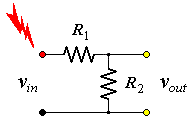
\includegraphics[scale = 2]{circuito sonda per alta tensione.png}
\end{figure}

sappiamo che: 

{
    \Large 
    \begin{equation}
        v_{out} = \frac{1}{1000} \cdot v_{in}
    \end{equation}
}

Invece la misura con il voltmetro collegato alla sonda: 

\begin{figure}[h]
    \centering
    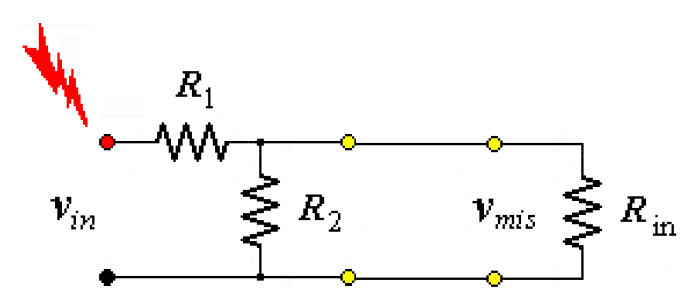
\includegraphics[scale = 0.6]{circuito di misura per sonda ad alta tensione.PNG}
\end{figure}

\newpage 

sappiamo che: 

{
    \Large 
    \begin{equation}
        v_{out}
        = 
        \frac{\frac{R_2 \cdot R_{in}}{R_2 + R_{in}}}{R_1 + \frac{R_2 \cdot R_{in}}{R_2 + R_{in}}} \cdot v_{in}
    \end{equation}
}

Facendo equagliare le due equazioni  e ponendo il valore nominale di $R_{in}$ di 10 M$\Omega$:

{
    \Large 
    \begin{equation}
        \begin{cases}
            v_{out} = \frac{1}{1000} \cdot v_{in}
            \\
            v_{out}
            = 
            \frac{\frac{R_2 \cdot R_{in}}{R_2 + R_{in}}}{R_1 + \frac{R_2 \cdot R_{in}}{R_2 + R_{in}}} \cdot v_{in}
            \\
            R_{in} = 10 M\Omega
        \end{cases}
        \rightarrow 
        R_2 = \frac{10}{9} M\Omega
    \end{equation}
}

data una $v_{in}$ qualsiasi, ricaviamo proprio $\frac{10}{9}$ M$\Omega$. \newline 

\newpage 

\subsection{Cautele e limitazioni d'uso}
\footnote{Slide della prof | SDME 4 Strumenti numerici indicatori - parte VII | pag 12\\  
Appunti | 2025-05-20 | pag 4 }

Le sonde che abbiamo descritto nelle sezioni precedenti come la sonda per alta tensione Fluke 80k-40, 
sono sonde in bassa potenza. \newline 

Da una semplice dimostrazione di elettrotecnica, sappiamo che: 

{
    \Large 
    \begin{equation}
        \begin{split}
        P &= V \cdot I
        \\
        &= R \cdot I^{2}
        \end{split}
    \end{equation}
}

Questa equazione ci da 3 gradi di liberta: P, R, I. \newline 

Se vogliamo che la potenza P sia molto bassa, avendo una tensione V molto alta, dobbiamo avere una corrente I molto bassa, 
che, per l'architettura del voltmetro che abbbiamo studiato, avere una corrente bassa è cosa buona e giusta per il suo funzionamento. \newline 

Se invece ragioniamo in corrente I, 
per avere P basso, ma avendo I molto alto, dobbiamo avere R che sia molto basso. \newline 

Inoltre il valore della resistenza degli stadi ingressi di tutti i voltmetri non è detto che siano uguali, quindi non possiamo fare le stesse considerazioni svolte precedentemente sulla sonda in alta tensione per i voltmetri. \newline 

Ad esempio in un voltmetro da banco come l'Agilent 34401A, 
la resistenza di ingresso cambia se si fa una misura in AC o in DC: 

\begin{itemize}
    \item $R_{in}$ in DC: 10 M$\Omega$
    \item $R_{in}$ in AC: 1 M$\Omega$
\end{itemize}

e non $\frac{10}{9}$ M$\Omega$ scritti precedentemente. \newline 

Se vogliamo misurare correnti I molto elevate, 
mantenendo la stessa architettura dello strumento di misura e quindi una P potenza molto bassa sullo stadio di ingresso dello strumento di misura, 
abbiamo bisogno di un resistore in parallelo allo strumento di misura che abbia valore nominale nettamente più piccolo rispetto al valore dello stadio di ingresso dello strumento di misura. \newline

Ecco spiegato il motivo dell'uso dei resistori di shunt. \newline 

\newpage 

\section{Resistore Shunt}
\footnote{Slide della prof | SDME 4 Strumenti numerici indicatori - parte VII | pag 13\\  
Appunti | 2025-05-20 | pag 4 }

Un modello disponibile sul mercato di resistore di shunt è il seguente: 

\begin{figure}[h]
    \centering
    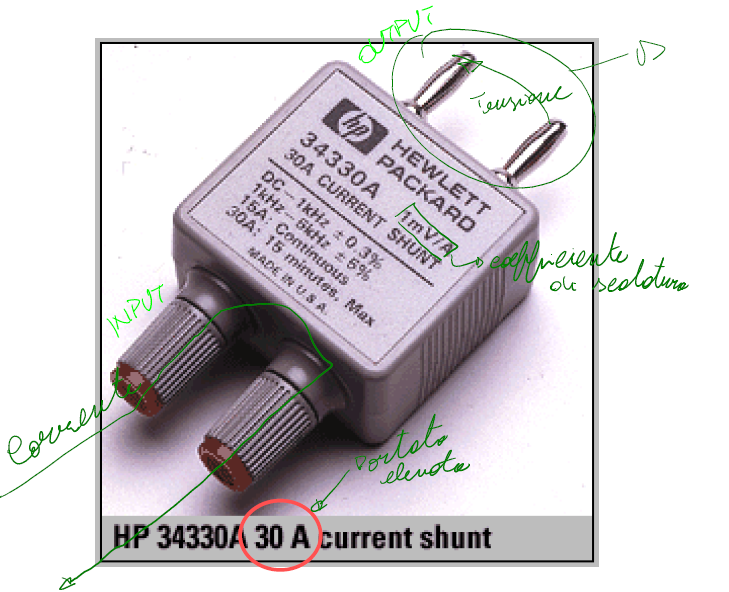
\includegraphics[scale = 1]{HP 34330A con annotazioni.PNG}
\end{figure}

Come scritto nelle annotazioni in figura, 
il resistore di shunt va messo in serie al carico in cui si vuole misurare una corrente molto elevata, 
la elevata corrente scorre tra i due bloccoli di input del resistore di shunt, 
invece nei pin di output, 
si avrà una tensione che rappresenta la corrente in ingresso ma scalata del coefficiente di scalatura. \newline 

Facendo dei semplici conti con la corrente massima $I_{max}$ che supporta questo modello di shunt, cioè 30 A,
e sapendo che il coefficiente di scalatura k è di $1 \left[\frac{mV}{A} \right]$, 
la tensione $v_{out}$ che avremo in uscita ad esso è di: 

{
    \Large 
    \begin{equation}
        \begin{split}
            v_{out} &= k \cdot I_{in}
            \\
            &= 1 \left[\frac{mV}{A} \right] \cdot 30 [A]
            \\
            &= 30 [mV]
        \end{split}
    \end{equation}
}

$v_{out}$ è una tensione molto bassa, che può essere misurata da un normale tester o da un voltmetro da banco. \newline 

\newpage 

\section{Partitore di corrente}
\footnote{Slide della prof | SDME 4 Strumenti numerici indicatori - parte VII | pag 14 - 17\\  
Appunti | 2025-05-20 | pag 4 - 5 }

I ragionamenti sono gli stessi per il partitore di tensione svolto precedentemente sulle sonde ad alta tensione, 
ma in questo caso ragioneremo usando la corrente. \newline 

Se si volesse misurare solo la corrente in un ramo, possiamo porre in serie al ramo l'amperometro, 
il cui valore noto del suo stadio di ingresso è di 1 $\Omega$: 

\begin{figure}[h]
    \centering
    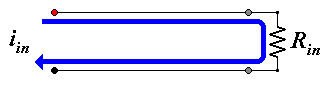
\includegraphics[scale = 1.5]{Misura di una corrente molto elevata ideale.png}
\end{figure}

Ma, in questo caso, essendo la corrente $i_{in}$ molto elevata, l'amperometro dovrebbe essere progettato per funzionare anche a queste correnti elevati. \newline 

L'amperometro non è stato progettato per funzionare a correnti molto elevate, soprattutto perchè si vuole proteggere l'operatore quando si utilizza lo strumento:
l'uomo può sopportare fino a 10 mA. \newline 

Per questo motivo che, in parallelo all'amperometro, viene posizionato un resistore di shunt: 

\begin{figure}[h]
    \centering
    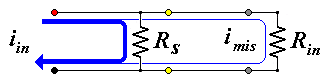
\includegraphics[scale = 1.5]{corrente elevata e resistore di shunt.png}
\end{figure}

in modo tale (vedi spessore delle frecce) che la maggior parte della corrente fluisca nella resistenza di shunt $R_s$ e non sulla resistenza dell'amperometro $R_{in}$. \newline 

La maggior parte della corrente scorre sulla resistenza di shunt $R_s$ perchè il suo valore nominale è di diversi gradi d'ordine inferiore rispetto a $R_{in}$. \newline 

In formule: 

{
    \Large 
    \begin{equation}
        R_s << R_{in}
    \end{equation}
}


Facendo i conti "carta e penna" e sapendo i valori noti di $R_s$ e $R_{in}$ tipici, rispettivamente, di un resisotre di shunt e di uno stadio di ingresso di un amperometro, 
avremo che: 

{
    \Large 
    \begin{equation}
        \begin{split}
            i_{mis}
            &= 
            \frac{R_s}{R_s + R_{in}} \cdot i_{in}
            \\
            &= 
            \frac{0.001 [\Omega]}{0.001 [\Omega] + 1 [\Omega]} \cdot i_{in}
            \\
            &=
            \frac{0.001}{1.001} \cdot i_{in}
            \\
            &\approx
            \frac{1}{1000} \cdot i_{in}
        \end{split}
    \end{equation}
}

Grazie alle osservazioni svolte sull'architettura dell'amperometro, 
sappiamo che $R_{in}$ varia in base alla portata dello strumento, 
inoltre è difficile quantificarla a causa di tutte le resistenze parassite dovuti ai fusibili, commutatori, boccole di ingresso e molti altri fattori che non stiamo qui ad elencare. \newline 

Sapendo che: 

{
    \Large 
    \begin{equation}
        i_{mis}
        =
        \frac{1}{1000} \cdot i_{in}
    \end{equation}
}

questa relazione non è sempre valida negli amperometri, 
quindi si sceglie di utilizzare in parallelo al resistore di shunt un voltmetro. \newline 

\newpage 

\section{Resistore "shunt" e voltmetro}
\footnote{Slide della prof | SDME 4 Strumenti numerici indicatori - parte VII | pag 19\\  
Appunti | 2025-05-20 | pag 5 }

Come visualizzato dalla seguente architettura: 

\begin{figure}[h]
    \centering
    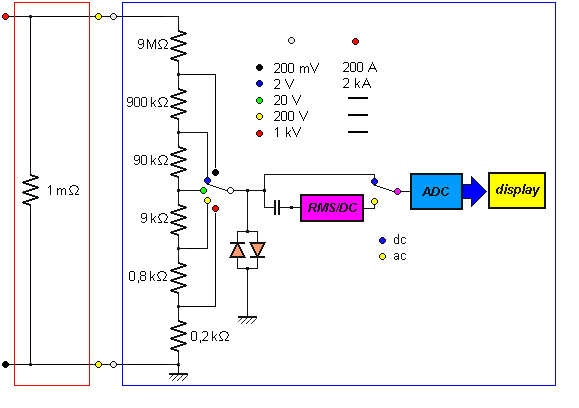
\includegraphics[scale = 1]{Resistore di shunt a 4 morsetti e voltmetro.png}
\end{figure}

questa è l'architettura di uno shunt a 4 morsetti collegato in parallelo ad un voltmetro. \newline 

In figura, lo shunt a quattro morsetti è tratteggiato in rosso, invece il voltmetro è tratteggiato in blu. \newline

Come si nota dalla figura, la resistenza di shunt ha un valore nominale di 1 m$\Omega$, che è di diversi gradi d'ordine più piccola della resistenza del voltmetro, 
che sappiamo ha un valore nominale costante, qualsiasi sia la portata scelta dello strumento, di $10 M\Omega$. \newline

La relazione fatta nella sezione precedente: 

\begin{figure}[h]
    \centering
    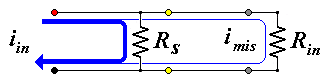
\includegraphics[scale = 1.5]{corrente elevata e resistore di shunt.png}
\end{figure}

{
    \Large 
    \begin{equation}
        \begin{split}
            R_s <&< R_{in}
            \\
            &\downarrow
            \\
            1 [m\Omega] <&< 10 [M\Omega]
        \end{split}
    \end{equation}
}

è valida, quindi la misura svolta sarà di buona qualità. \newline

Diremo che la misura è di pessima qualità quando $R_{in}$ è simile a $R_s$, quindi $R_s$, in quel caso, sarebbe una resistenza parassita che peggiora la qualità della misura. \newline 


L'obbiettivo di questa architettura shunt + voltmetro è quello di far circolare la corrente incognita su un resistore noto di valore piccolo 
e poi misurare la caduta di tensione. \newline 

\newpage 

\section{"Shunt" esterno per voltmetro}
\footnote{Slide della prof | SDME 4 Strumenti numerici indicatori - parte VII | pag 20\\  
Appunti | 2025-05-20 | pag 5 }

Come si vede dalle specifiche tecniche dello shunt reale di esempio: 

\begin{figure}[h]
    \centering
    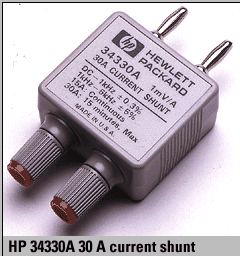
\includegraphics[scale = 1.5]{HP current shunt.png}
\end{figure}


essendo un componente reale, il suo comportamento varierà in base al grandezza da misurare. \newline 

Il campo di misura è da DC (cioè Hz = 0) fino a correnti AC fino a 5 kHz, dove, in base alla frequenza, lo shunt darà una sua incertezza: 

\begin{itemize}
    \item DC - 1 kHz, l'incertezza della tensione in uscita è di $\pm 0.3 \%$
    \item 1 kHz - 5 kHz, l'incertezza della tensione in uscita è di $\pm 5 \%$
\end{itemize}

Questi valori di incertezza sono buoni per correnti elettriche perchè andremo a lavorare con correnti a 50 Hz. \newline 

Inoltre, la portata può variare: 

\begin{itemize}
    \item 15 A continui, cioè sempre 
    \item 30 A solo per 15 minuti, sennò lo shunt emette troppo calore e/o si brucia il componente e/o non riesce a garantire l'incertezza indicata
\end{itemize}

Si svolge una misura a quattro morsetti per evitare gli effetti delle resistenze parassite dei cavi e dei connettori. \newline 

\newpage 

\section{"Shunt" esterno per elevate correnti}
\footnote{Slide della prof | SDME 4 Strumenti numerici indicatori - parte VII | pag 21\\  
Appunti | 2025-05-20 | pag 5 }

Se si vuole misurare delle correnti molto elevate, fisicamente lo shunt deve essere differente rispetto all'HP 34330A. \newline 

Un esempio fisico di uno shunt per elevate correnti: 

\begin{figure}[h]
    \centering
    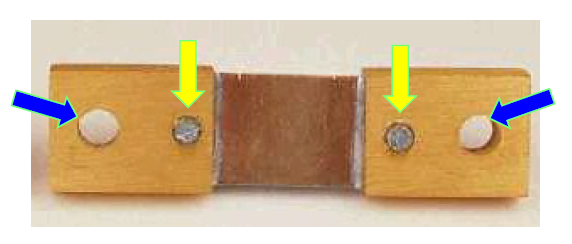
\includegraphics[scale = 1]{shunt per elevate correnti.PNG}
\end{figure}

dove, nella figura, le frecce indicato indicano i 4 morsetti dello shunt (si è passato dalle boccole ai punti come questi). \newline 

Le caratteristiche di questo tipo di shunt sono le seguenti: 

\begin{itemize}
    \item $R_s$ = 0.25 [m$\Omega$]
    \item costante di lettura = 0.25 $[\frac{mV}{A}]$
    \item portata: 300 A continui
\end{itemize}

Questo tipo di realizzazione è molto più grossolana, ma per correnti molto elevate va benissimo. \newline 

Generalmente questo tipo di shunt si monta all'interno di un quadro elettrico. \newline 

\newpage 

\section{Accoppiamento in alternata (AC - Alternated Coupling ): trasformatori di misura - TV e TA}
\footnote{Slide della prof | SDME 4 Strumenti numerici indicatori - parte VII | pag 22\\  
Appunti | 2025-05-20 | pag 5 - 6 | 2025-05-26 | pag 1}

In AC, o in alternata, per portate elevate, si sfruttano i principi dei trasformatori, in particolare dei loro rapporti di conversione, 
cioè il rapporto tra il numero di spire del primario e il numero di spire del secondario. \newline 

\begin{tcolorbox}
    Un piccolo ripasso al volo del pricipio di funzionamento dei trasformatori: \\
    \url{https://www.edutecnica.it/elettrotecnica/trasformatore/trasformatore.htm}
\end{tcolorbox}

Si utilizzano dei Trasformatori Voltmetrici (o abbreviato TV) per misurare le tensioni elevate, 
oppure si utilizzano dei Trasformatori Amperometrici (o abbrevuato TA) per misurare le correnti elevate. \newline 

Di seguito dei modelli acquistabili di TV e TA di misura per media tensione (10 - 30 kV): 

\begin{figure}[h]
    \centering
    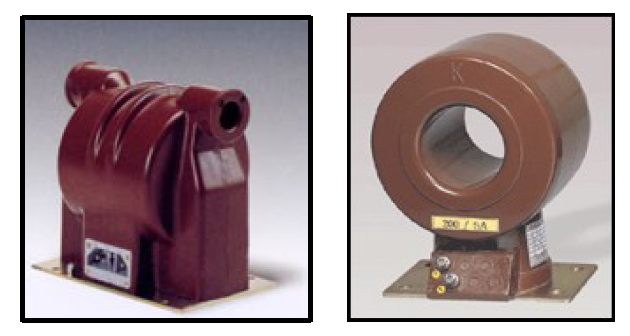
\includegraphics[scale = 1]{TV e TA.PNG}
\end{figure}

Dal corso di fondamenti di elettromagnetismo, sappiamo che nei trasformatori il modulo e la fase delle grandezze sono diversi tra primario e secondario, 
quindi i TA ed i TV produrranno degli errori di fase e di modulo. \newline 

\newpage 

\subsection{Traformatori di misura per alta tensione 60 - 132 kV}
\footnote{Slide della prof | SDME 4 Strumenti numerici indicatori - parte VII | pag 23\\  
Appunti | 2025-05-26 | pag 1}

Altri esempi fisici di TA e TV, in questo caso per l'alta tensione: 

\begin{figure}[h]
    \centering
    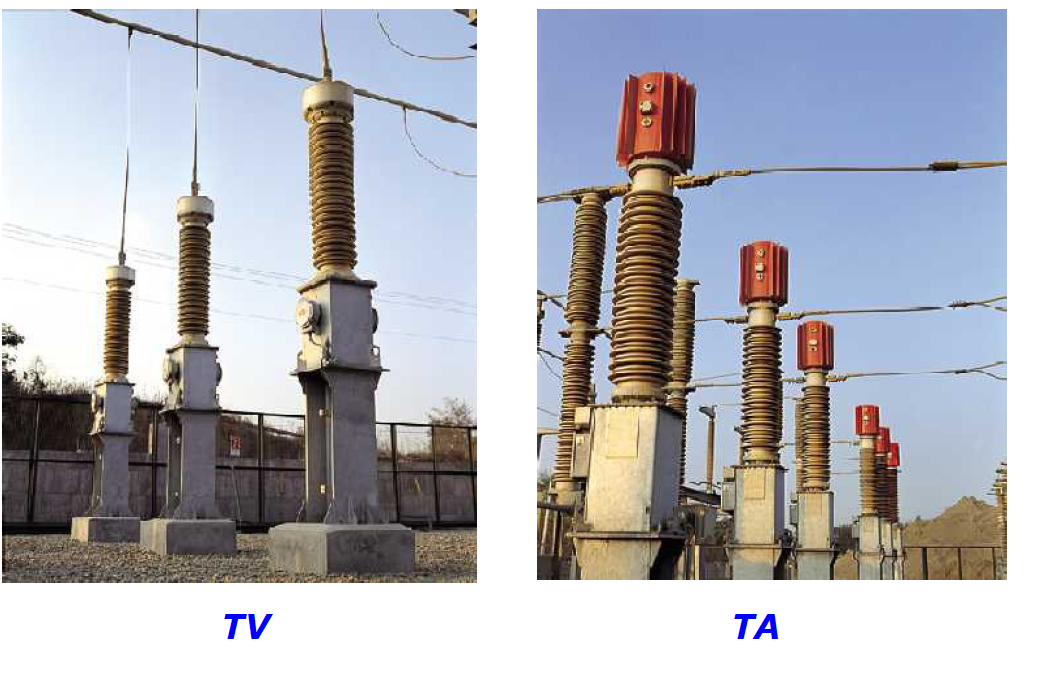
\includegraphics[scale = 0.5]{TV e TA per l'alta tensione.PNG}
\end{figure}

\begin{tcolorbox}
Un esempio in commercio di TA per alta tensione:\\
\url{https://www.hitachienergy.com/it/it/products-and-solutions/instrument-transformers/current-transformers-and-sensors/tg-72-5-800-kv}     
\end{tcolorbox}


\newpage 

\subsection{Trasformatore Voltmetrico TV}
\footnote{Slide della prof | SDME 4 Strumenti numerici indicatori - parte VII | pag 24\\  
Appunti | 2025-05-26 | pag 1}

Dal corso di fondamenti di elettromagnetismo, sappiamo che possiamo rappresentare un trasformatore ideale in questa maniera: 

\begin{figure}[h]
    \centering
    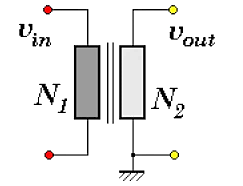
\includegraphics[scale = 1]{Trasformatore ideale.png}
\end{figure}

di cui possiamo scrivere la seguente relazione: 

{
    \Large 
    \begin{equation}
        v_{out}
        \approx
        \frac{N_2}{N_1} \cdot v_{in}
    \end{equation}
}

dove: 

\begin{itemize}
    \item $N_1$ e $N_2$ sono, rispettivamente, il numero di spire del primario e del secondario 
    \item $v_{in}$ è la tensione di ingresso, cioè la tensione ai capi del primario 
    \item $v_{out}$ è la tensione in uscita, cioè la tensione ai capi del secondario
\end{itemize}

Inoltre, dalla figura notiamo che ci sono due barrette parallele tra $N_1$ e $N_2$ perchè le linee di campo sono parallele. \newline 

Nella relazione tra $v_{out}$ e $v_{in}$ scriviamo $\approx$ perchè non tutte le linee di campo si concentrano tra primario e secondario: 
ci sarà più intensità di campo tra primario e secondario, ma parte verrà dispersa. \newline 

Inoltre, dalla relazione tra $v_{out}$ e $v_{in}$ si può notare che, se $N_1 > N_2$, la tensione $v_{in}$ viene scalata di un fattore $\frac{N_2}{N_1}$, quindi $v_{out}$ sarà minore di $v_{in}$. \newline 

Per quanto riguarda le tensioni molto elevate, dal circuito del trasformatore, notiamo che 
$v_{in}$ non è una tensione con la messa a terra, rispetto a $v_{out}$ dove è presente la terra dello strumento: 
questa caratteristica è molto comoda quando si vanno a fare misure in impianti ad alta tensione perchè è difficile svolgere una misura con la terra. \newline

\newpage 

\subsection{Trasformatore Amperometrico TA}
\footnote{Slide della prof | SDME 4 Strumenti numerici indicatori - parte VII | pag 25, 27\\  
Appunti | 2025-05-26 | pag 1 }

Per quanto riguarda il Trasformatore Amperometrico TA, abbiamo anche lì un trasformatore dove: 

\begin{figure}[h]
    \centering
    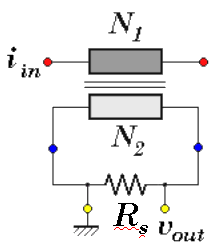
\includegraphics[scale = 1]{Traformatore ideale corrente.png}
\end{figure}

Ponendo un piccolo resistore di shunt $R_s$ nel secondario, è possibile far circolare una piccola corrente $i_2$ del valore di:

{
    \Large 
    \begin{equation}
        i_2 \approx \frac{N_1}{N_2} \cdot i_{in}
    \end{equation}
}

Inoltre, nel TA, possiamo misurare la tensione ai capi di $R_s$, che vale: 

{
    \Large
    \begin{equation}
        \begin{split}
        v_{out} &\approx R_s \cdot i_2
        \\
        &\approx R_s \cdot \left( \frac{N_1}{N_2} \cdot i_{in} \right)
        \end{split}
    \end{equation}
}

Dalla seguente relazione, $v_{out}$ è proporzionale a $i_{in}$. \newline 

Visualizzando il circuito di misura del TA: 

\begin{figure}[h]
    \centering
    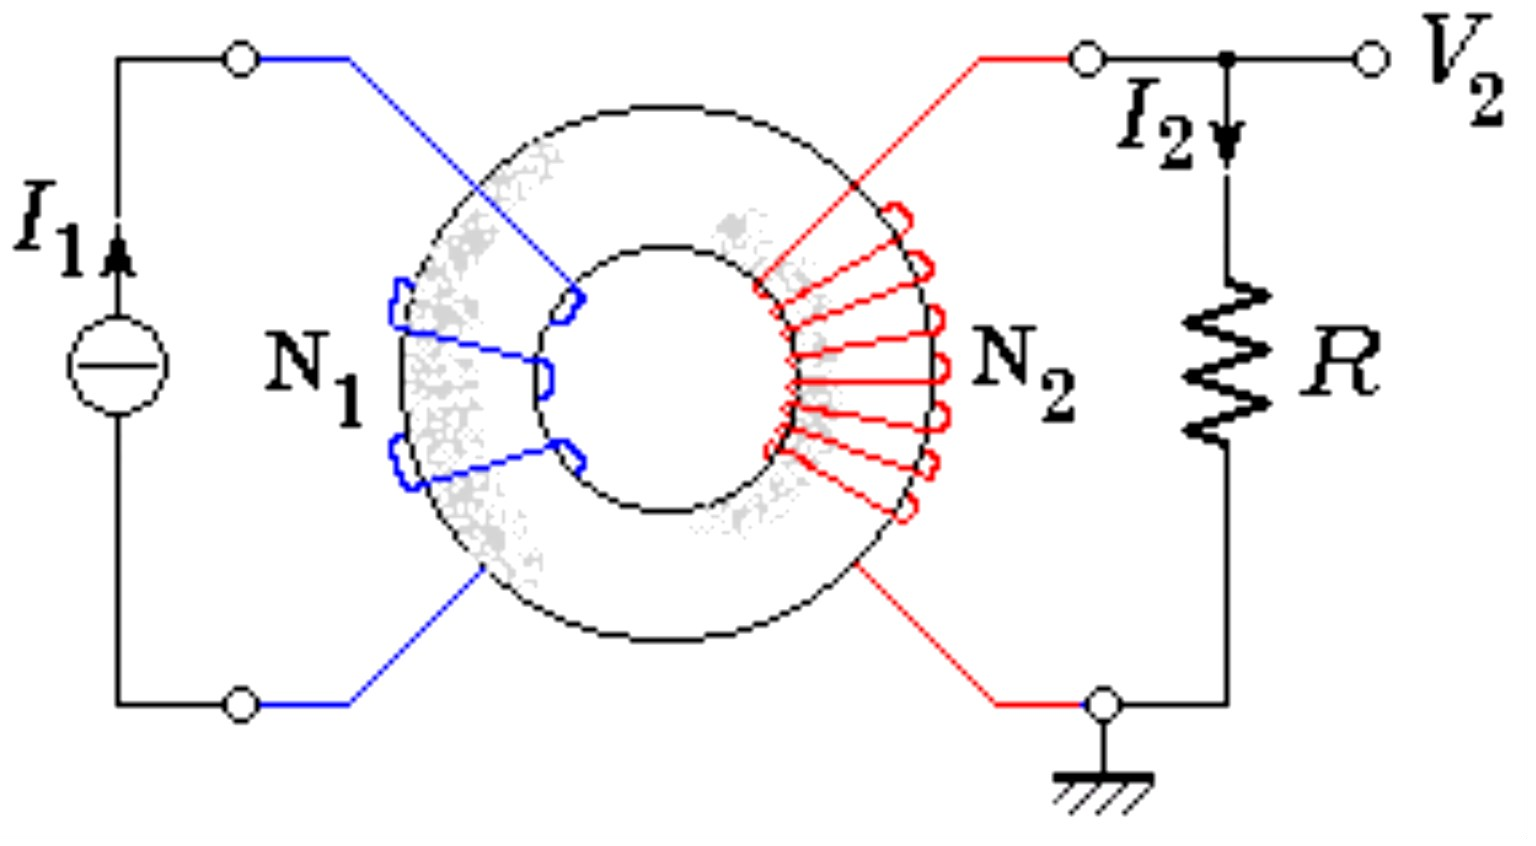
\includegraphics[scale = 0.5]{Spire nel TA.png}
\end{figure}

il numero delle spire può essere causa di incertezza. \newline 

Per questo motivo, i trasformatori di misura sono ben realizzati e utilizzati come da manuale. \newline 


\newpage 

\subsection{Il TA non deve operare con il secondario aperto}
\footnote{Slide della prof | SDME 4 Strumenti numerici indicatori - parte VII | pag 26\\  
Appunti | 2025-05-26 | pag 1 - 2} 

Come scritto nel titolo, il TA non deve operare con il secondario aperto: 
bisogna avere sempre un resistore per far circolare una corrente $i_2$ nel secondario. \newline 

Se non si predispone di una resistenza, i TA predispongono di questo interruttore a coltello (cerchiato in giallo in figura): 

\begin{figure}[h]
    \centering
    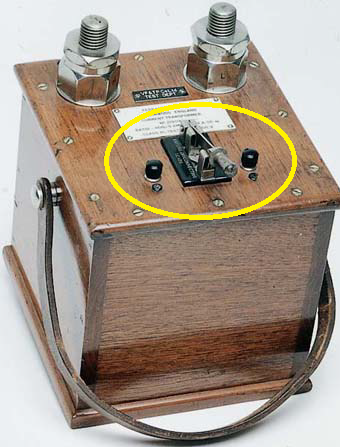
\includegraphics[scale = 1]{Intettuttore a coltello nei TA.png}
\end{figure}

che se abbassato, impone una piccola resistenza, chiude il circuito del secondario quindi fa circolare una corrente anche nel secondario. \newline  

\newpage 

\section{Il TA con una sola spira}
\footnote{Slide della prof | SDME 4 Strumenti numerici indicatori - parte VII | pag 28\\  
Appunti | 2025-05-26 | pag 2} 

Dalla fisica, dall'elettromagnetismo e dall'elettrotecnica, il numero $N_1$ di spire del primario e il numero $N_2$ di spire del secondario può essere qualsiasi, 
basta che il loro rapporto $\frac{N_2}{N_1}$ rimanga costante. \newline 

Siccome, con un trasformatore TA si interrompe il circuito sotto misura e negli stadi successivi ci saranno altre cause di incertezza, 
si sceglie, per semplicità e per abbassare l'incertezza, di fare solo 1 spira nel primario, e nel secondo N spire che servono per mantenere costante il rapporto $\frac{N_2}{N_1}$. \newline 

Questo semplice concetto, permette di realizzare fisicamente dei TA di diversa geometria. \newline 

Utilizzando questo concetto, si possono realizzare dei TA a barra passante per i cavi unipolari, che fisicamente circondano il cavo sotto misura: 

\begin{figure}[h]
    \centering
    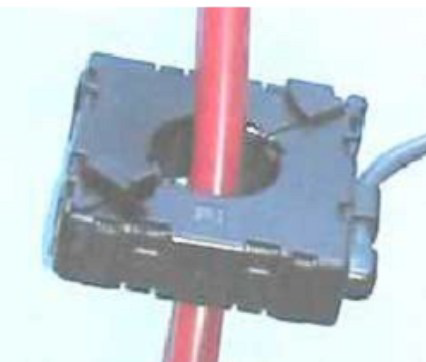
\includegraphics[scale = 0.5]{cavo unipolare.png}
\end{figure}

e si può schematizzzare il circuito così: 

\begin{figure}[h]
    \centering
    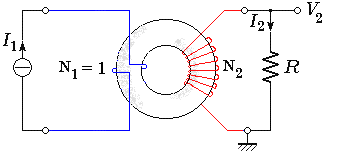
\includegraphics[scale = 1.5]{cavo unipolare schema circuitale.png}
\end{figure}

Oppure, in campi industriali, si impiegano questi TA "a barra passante": 

\begin{figure}[h]
    \centering
    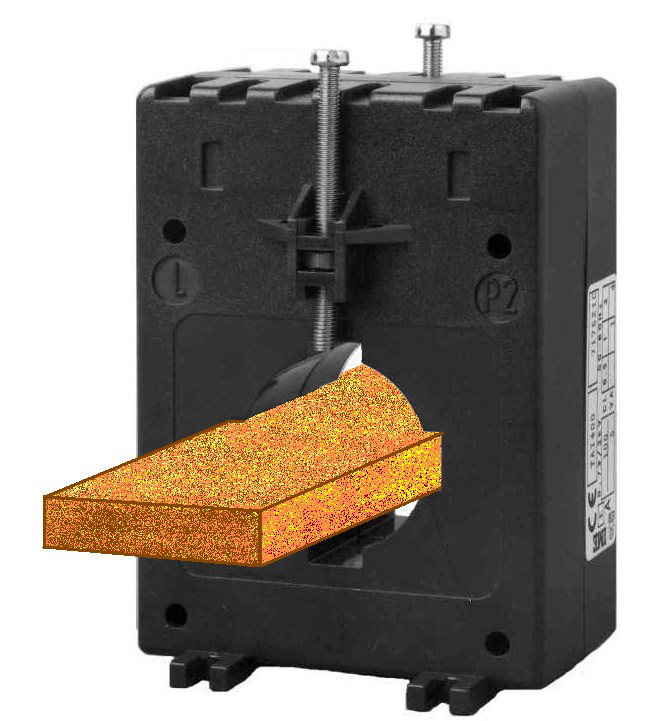
\includegraphics[scale = 0.4]{TA a barra passante ambito industriale.png}
\end{figure}

\newpage 

e si può schematizzare il circuito così: 

\begin{figure}[h]
    \centering
    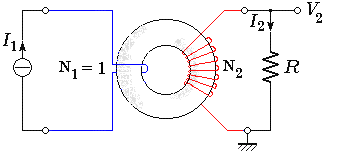
\includegraphics[scale = 1.5]{TA a barra passante ambito industriale schema circuitale.png}
\end{figure}

oppure: 

\begin{figure}[h]
    \centering
    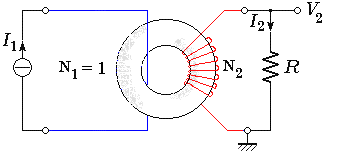
\includegraphics[scale = 1.5]{TA a barra passante ambito industriale schema circuitale parte 2.png}
\end{figure}

Vengono impiegati questi tipi di TA perchè i cavi, negli impianti industriali, sono di grosse dimensioni e standardizzati, 
quindi non possiamo interrompere il circuito come si farebbe a casa con due cavi jumper, un led e un Arduino. \newline 

\newpage

\subsection{TA "a pinza" (nucleo apribile) }
\footnote{Slide della prof | SDME 4 Strumenti numerici indicatori - parte VII | pag 30 - 33\\  
Appunti | 2025-05-26 | pag 2 - 3}

Sempre con lo stesso principio, sono disponibili in commercio i TA "a pinza" apribili: 

\begin{figure}[h]
    \centering
    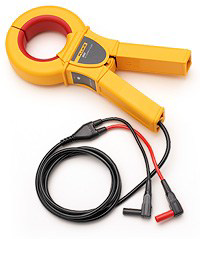
\includegraphics[scale = 1]{TA a pinza apribile.png}
\end{figure}

dove in uscita abbiamo dei connettori a banana che devono essere collegati ad un amperometro. \newline 

Il circuito schematizzato è: 

\begin{figure}[h]
    \centering
    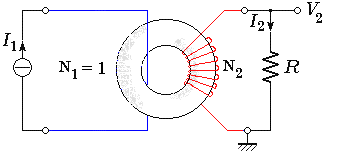
\includegraphics[scale = 1.5]{TA a barra passante ambito industriale schema circuitale parte 2.png}
\end{figure}

Altri tipi di TA a pinza sono questi: 

\begin{figure}[h]
    \centering
    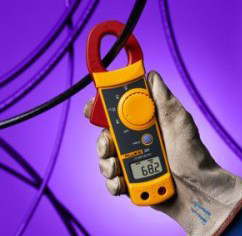
\includegraphics[scale = 1]{TA a pinza apribile con amperometro incluso.png}
\end{figure}

in cui è già incluso un circuito di voltmetro. \newline 

Oppure semplici TA a pinza di diverse dimensioni, a seconda del cavo da misurare: 

\newpage 

\begin{figure}[h]
    \centering
    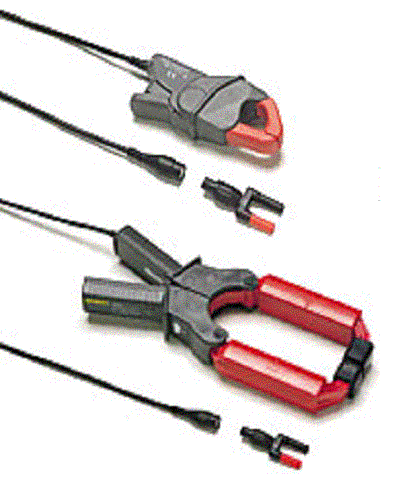
\includegraphics[scale = 0.5]{TA di diversa geometria.png}
\end{figure}

Le caratteristica di un tipico TA a pinza sono le seguenti: 

\begin{itemize}
    \item da 1 A a 400 A in valore efficace con picchi di 1 kA
    \item da 5 Hz a 20 kHz 
    \item sensibilità 1 $\frac{mA}{A}$ 
    \item incertezza di modulo $\pm 2 \% $ da 45 Hz a 400 Hz (frequenze in ambito industriale)
\end{itemize}

L'incertezza del modulo è molto elevata perchè la pinza è apribile, quindi il secondario non riesce a raccogliere e a concentrate tutte le linee di campo magnetico. \newline 

\newpage 

\subsection{TA flessibile "a bobina di Rogowski"}
\footnote{Slide della prof | SDME 4 Strumenti numerici indicatori - parte VII | pag 34 - 36\\  
Appunti | 2025-05-26 | pag 3}

Stesso principio di TA a pinza, ma in cui il nucleo è flessibile: 

\begin{figure}[h]
    \centering
    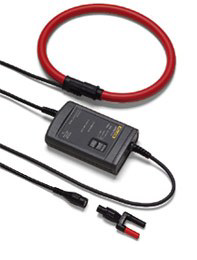
\includegraphics[scale = 1]{TA flessibile.png}
\end{figure}

Vengono anche essi utilizzati in ambito industriale, in cui non è possbile interrompere il circuito perchè i cavi sono grossi e standardizzati. \newline 

Sfrutta il principio di Faraday: 

\begin{figure}[h]
    \centering
    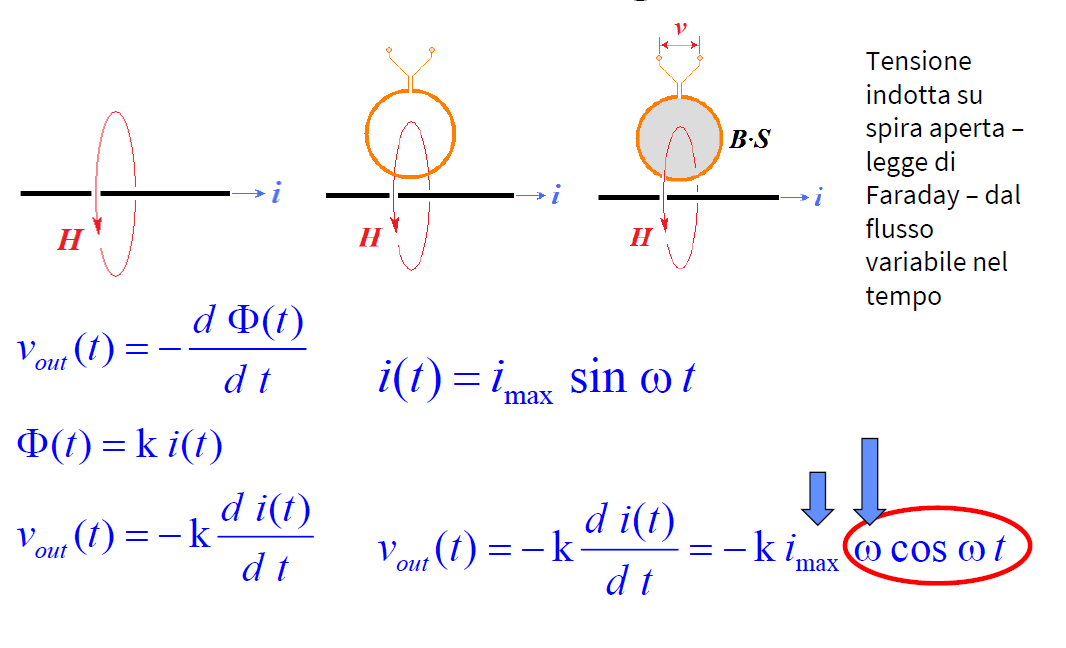
\includegraphics[scale = 0.6]{principio di funzionamento bobina di Rogowski.PNG}
\end{figure}

\newpage 

FINE PROGRAMMA A.A. 2024/2025 \newline 

BUON ESAME !!!


\begin{figure}[h]
    \centering
    
\includegraphics[scale = 0.4]{meme.jpg}
\end{figure}



